\documentclass[aspectratio=169]{beamer}

% 16:9 has textwidth 398.3386pt
% 4:3 has textwidth 307.28987pt.

\usetheme[numbering=none, progressbar=frametitle]{metropolis}
\usepackage[lf]{FiraSans}
\usepackage{bm}
\usepackage{booktabs}
\usepackage{siunitx}
\bibliographystyle{plainnat}
\graphicspath{{fig/}}

\pagenumbering{gobble}


\author{Jack Walton}
\title{Bayesian Statistics in Astrophysics}
\date{October 23, 2019}

\begin{document}

\maketitle

\begin{frame}{Disclaimer}
  \begin{columns}
    \begin{column}{0.5\textwidth}
      I am \emph{not} talking about my own research because:
      \begin{enumerate}
        \item \emph{Most} of you saw me talk at the applied PGR conference at the end
              of June
        \item I have no new results since June (I suspended studies for 3 months
              over summer)
      \end{enumerate}
    \end{column}
    \begin{column}{0.5\textwidth}
      \begin{figure}
        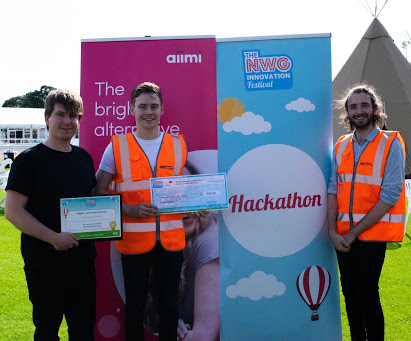
\includegraphics[width=\textwidth]{win.jpg}
        \caption{No new research here\ldots}
      \end{figure}
    \end{column}
  \end{columns}
\end{frame}

\begin{frame}{Table of contents}
  \tableofcontents
\end{frame}

\section{Bayesian \& frequentist statistics}

\begin{frame}{Frequentist statistics}
  \begin{itemize}
    \item This approach to statistics will be familiar to most
    \item Think $p$-values, hypothesis testing, confidence intervals etc.
    \item However, it is not the only statistical framework (nor is it the
          focus of this talk\ldots)
  \end{itemize}
\end{frame}

\begin{frame}{Bayesian vs. frequentist statistics}
  The difference between Bayesians and frequentists lies in the interpretation
  of probability\ldots

  For a \emph{frequentist}:\\\vspace{0.25cm}
  \begin{quote}
    {\normalfont An event's probability is the limit of its \alert{relative
        frequency in many trials}}
  \end{quote}

  For a \emph{Bayesian}:\\\vspace{0.25cm}
  \begin{quote}
    {\normalfont An event's probability is a \alert{degree of belief}}
  \end{quote}
\end{frame}

\begin{frame}{\emph{Why} Bayesian?}
  \begin{itemize}
    \item Philosophically aligns with how we practice science: \emph{updating}
          our \emph{beliefs} in light of \emph{new evidence}
    \item Allows the inclusion of expert information through a \emph{prior
            distribution}
    \item For events that only occur once, how appropriate is a methodology
          which relies on repeatability?
  \end{itemize}
\end{frame}

\begin{frame}{Bayes' Theorem}
  \begin{columns}
    \begin{column}{0.6\textwidth}
      \vspace{1em}
      \begin{equation*}
        \pi(\theta \,|\,\bm{x}) = \frac{\pi(\theta)\,L(\bm{x}\,|\,\theta)}{\int_{\Theta} \pi(\bm{x}\,|\,\theta)\, \text{d}\theta}
      \end{equation*}
      \begin{itemize}
        \setlength\itemsep{1em}
        \item $\pi(\theta)$ represents our \alert{prior} beliefs
        \item $L(\bm{x}\,|\,\theta)$ is the likelihood of observing $\bm{x}$ given the model \& parameters $\theta$
        \item $\int_{\Theta} \pi(\bm{x}\,|\,\theta)\, \text{d}\theta$ is the normalising constant (probability of $\bm{x})$
        \item $\pi(\theta \, | \, \bm{x})$ represents our \alert{posterior} beliefs
      \end{itemize}
    \end{column}
    \begin{column}{0.4\textwidth}
      \begin{figure}
        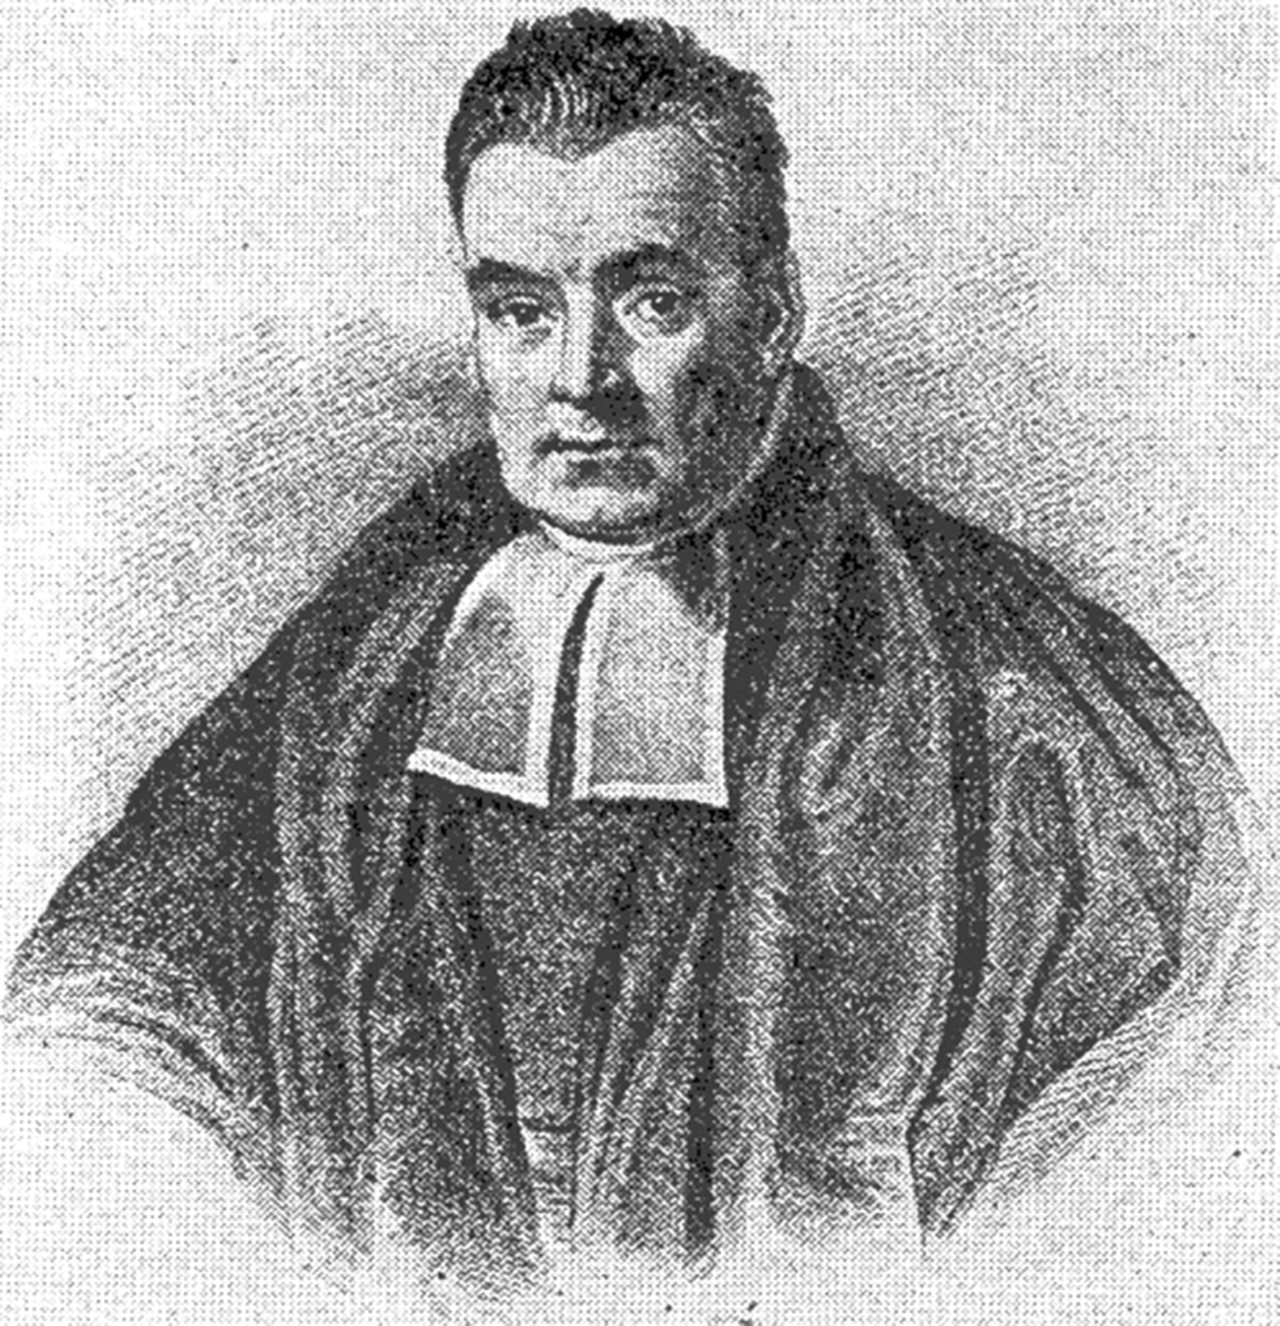
\includegraphics[width=\textwidth]{baes.jpg}
        \caption{Purportedly Bayes}
      \end{figure}
    \end{column}
  \end{columns}
\end{frame}

% naughty
\setcounter{figure}{1}

\begin{frame}{Bayes' Theorem}
  \begin{columns}
    \begin{column}{0.6\textwidth}
      Typically, $\int_{\Theta} \pi(\bm{x}\,|\,\theta)\, \text{d}\theta$ is \emph{very} difficult to compute.\\\vspace{0.5cm}

      Instead we often consider:

      \begin{align*}
        \pi(\theta\,|\,\bm{x}) & \propto \pi(\theta) \times L(\bm{x}\,|\,\theta) \\
        \text{posterior}       & \propto \text{prior} \times \text{likelihood}
      \end{align*}
    \end{column}
    \begin{column}{0.4\textwidth}
      \begin{figure}
        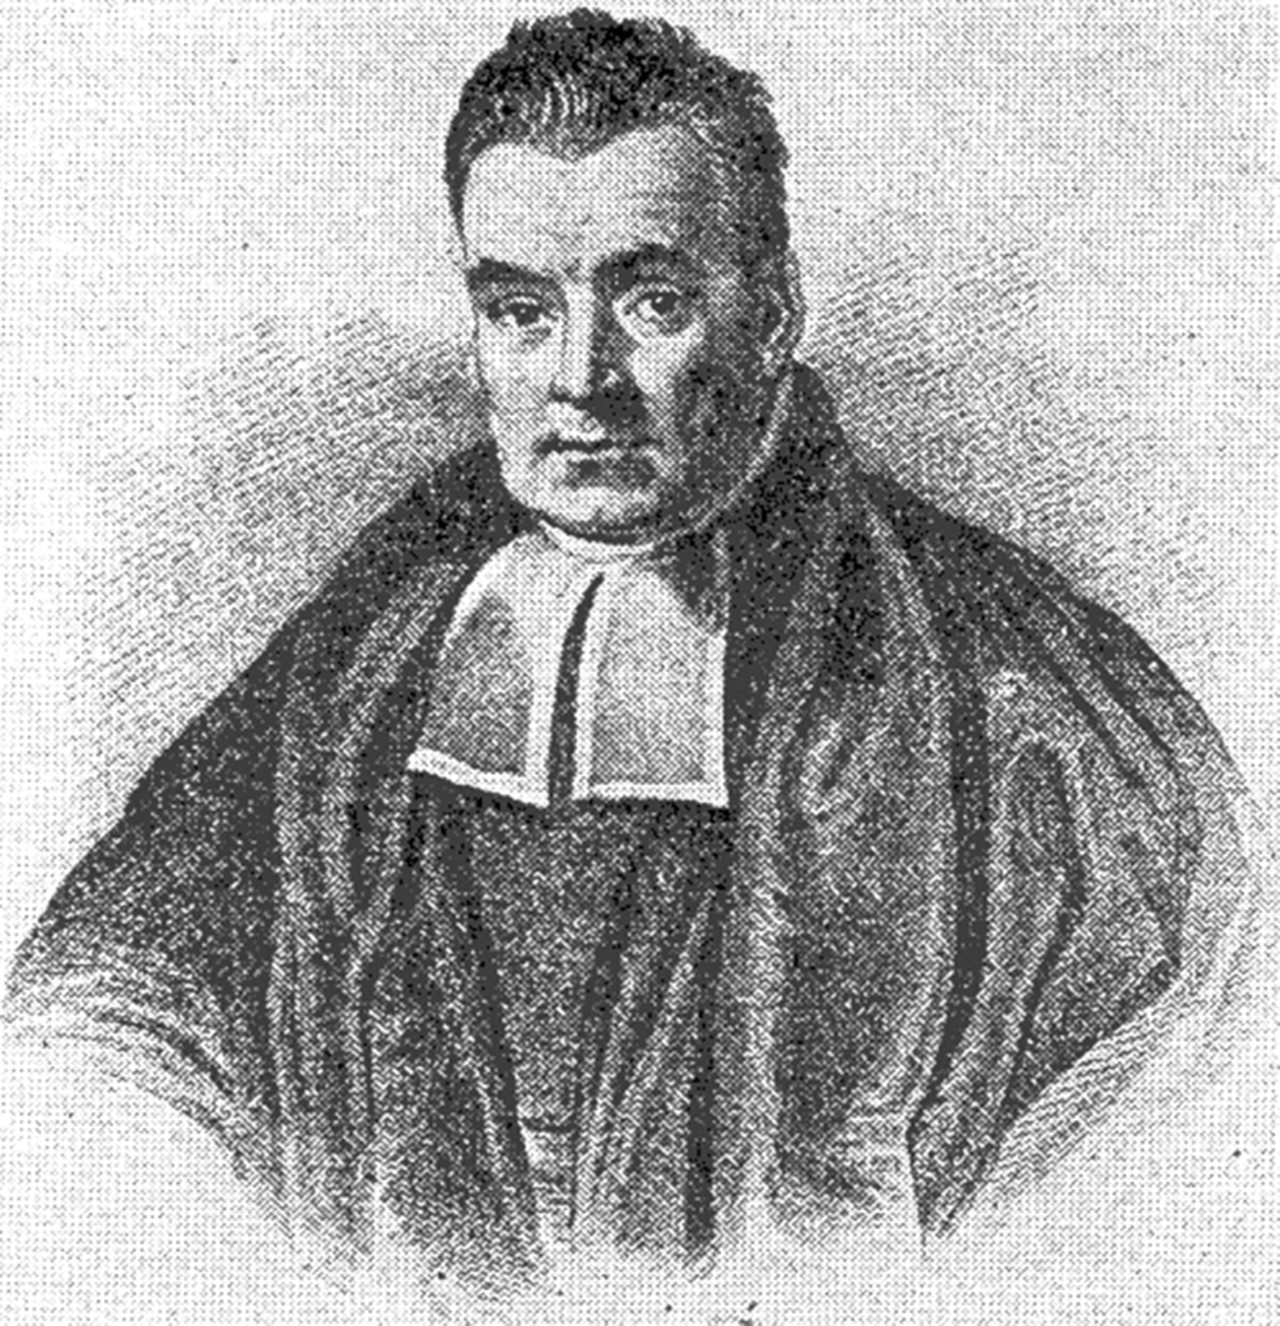
\includegraphics[width=\textwidth]{baes.jpg}
        \caption{Purportedly Bayes}
      \end{figure}
    \end{column}
  \end{columns}
\end{frame}

\begin{frame}{MCMC}
  \begin{itemize}
    \item MCMC --- Markov Chain Monte Carlo
    \item Class of algorithms used to sample from probability densities
    \item We can use them to sample from $\pi(\theta \, | \, \bm{x})$, our
          posterior distribution
    \item Avoids the computation of $\pi(\bm{x})$
  \end{itemize}
\end{frame}

\begin{frame}{Stan}
  \begin{columns}
    \begin{column}{0.6\textwidth}
      \begin{itemize}
        \item Probabilistic programming language wrote in C++. Accessed via
              interfaces with Python, R, Matlab, Julia\ldots
        \item Stan implements current state-of-the-art MCMC algorithms
        \item Named after Stanislaw Ulam, a mathematician and nuclear physicist and
              pioneer of Monte-Carlo methods.
      \end{itemize}
    \end{column}
    \begin{column}{0.4\textwidth}
      \begin{figure}
        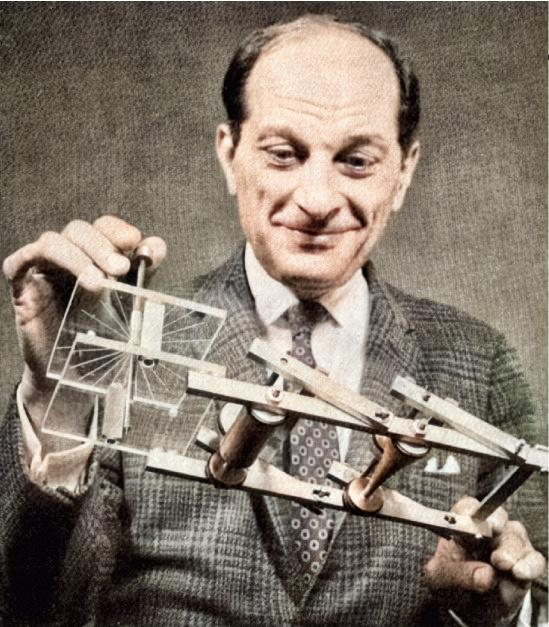
\includegraphics[width=0.9\textwidth]{stan.jpg}
        \caption{Stanislaw \& the FERMIAC}
      \end{figure}
    \end{column}
  \end{columns}
\end{frame}

\section{Sunspot occurrence: a case study}

\begin{frame}{What \emph{are} sunspots?}
  \begin{columns}
    \begin{column}{0.6\textwidth}
      \begin{itemize}
        \item Dark regions which appear on the surface of the sun
        \item Cooler areas, caused by concentrations of magnetic field flux
        \item Precursor to more dramatic events such as solar flares and
              coronal mass ejections
        \item Significant concern for astronauts living in space, airline
              passengers on polar routes and satellite engineers
      \end{itemize}
    \end{column}%
    \begin{column}{0.4\textwidth}
      \begin{figure}
        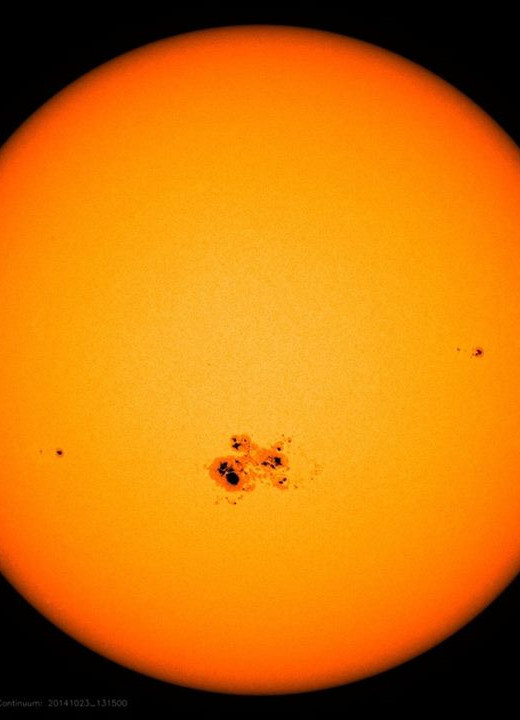
\includegraphics[width=0.8\textwidth]{sun.jpg}
        \caption{Sunspots}
      \end{figure}
    \end{column}
  \end{columns}
\end{frame}

\begin{frame}{Data}
  \begin{columns}
    \begin{column}{0.5\textwidth}
      We shall use the mean annual data for the International Sunspot number,
      under the responsibility of the Royal Observatory in Belgium since 1980.
    \end{column}
    \begin{column}{0.5\textwidth}
      \vspace{1em}
      \begin{figure}
        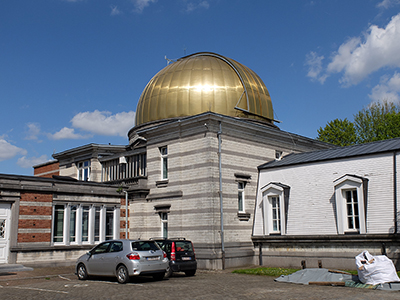
\includegraphics[width=\textwidth]{belgium.JPG}
        \caption{Royal observatory of Belgium}
      \end{figure}
    \end{column}
  \end{columns}
\end{frame}

\begin{frame}{Normal $AR(1)$ model}
  \begin{align*}
    S_{t} \sim Normal(\mu_t, \sigma^2)    & \\
    \mu_t = \varphi_1 + \varphi_2 S_{t-1} &
  \end{align*}

  Given the observed data can we infer the parameters $\varphi_1$,
  $\varphi_2$ and $\sigma$?
\end{frame}

\begin{frame}{Results: summary}
  \centering
  \begin{table}
    \input{fitting/out/norm.tab}
    \caption{Summary of posterior samples after running Stan for $10\,000$ iterations (3 seconds).}
  \end{table}
\end{frame}

\begin{frame}{Results: posterior densities}
  \begin{figure}
    \centering
    \includegraphics{fitting/out/norm_kde.pdf}
  \end{figure}
\end{frame}

\begin{frame}{Results: posterior predictives}
  \vspace{-0.3cm}
  \begin{figure}
    \centering
    \includegraphics{fitting/out/norm_post_fit.pdf}
  \end{figure}
\end{frame}

\begin{frame}{Negative Binomial $AR(1)$ model}
  \begin{align*}
    S_{t} \sim NB(p_t, \theta)                 & \\
    p_t = \theta / (\theta + \mu_t)            & \\
    \log(\mu_t) = \varphi_1 + \varphi_2S_{t-1} &
  \end{align*}
  Given the observed data can we infer the parameters $\varphi_1$,
  $\varphi_2$ and $\theta$?
\end{frame}

\begin{frame}{Results: summary}
  \begin{table}
    \centering
    \input{fitting/out/neg_bin.tab}
    \caption{Summary of posterior samples after running Stan for $10\,000$ iterations (30 seconds).}
  \end{table}
\end{frame}

\begin{frame}{Results: posterior densities}
  \begin{figure}
    \centering
    \includegraphics{fitting/out/norm_kde.pdf}
  \end{figure}
\end{frame}

\begin{frame}{Results: posterior predictives}
  \vspace{-0.3cm}
  \begin{figure}
    \centering
    \includegraphics{fitting/out/neg_bin_post_fit.pdf}
  \end{figure}
\end{frame}

\begin{frame}{Conclusion}
  \begin{itemize}
    \item Modern computing power is making Bayesian methodologies more accessible
    \item Many `black-box' MCMC implementations make inference pain-free
    \item The inclusion of prior information can be useful for astronomical
          events which have limited observational data
  \end{itemize}
\end{frame}

\begin{frame}{References}
  \nocite{hilbe2017bayesian}
  \bibliography{references.bib}
\end{frame}

\begin{frame}[standout]
  Thanks
\end{frame}

\end{document}
